% Figure: Contravariant Orders — Causal filtration vs Stratum filtration
% Left column: causal order (log position). Right column: stratum order.
% Crossing lines show the contravariance.
\begin{figure}[t]
\centering
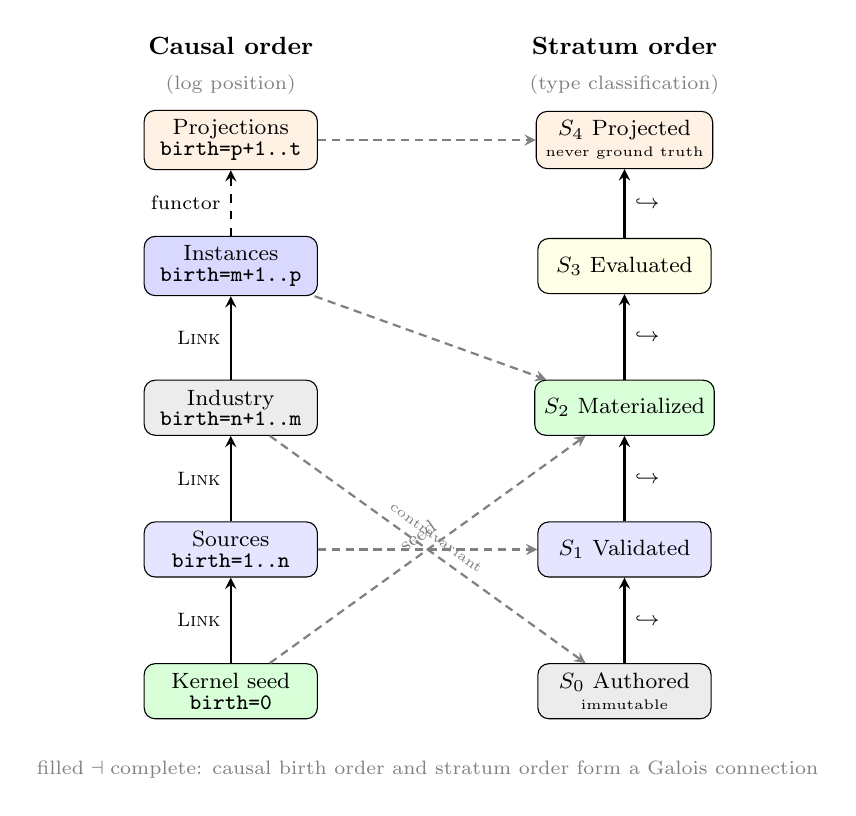
\begin{tikzpicture}[
  node/.style={draw, rounded corners, minimum width=2.2cm, minimum height=0.7cm, align=center, font=\footnotesize},
  arrow/.style={->, thick, >=stealth},
  cross/.style={->, thick, >=stealth, densely dashed, gray},
  lbl/.style={font=\scriptsize},
  col/.style={font=\small\bfseries}
]

% Column headers
\node[col] at (-2.5, 8.2) {Causal order};
\node[col] at (2.5, 8.2) {Stratum order};
\node[font=\scriptsize, text=gray] at (-2.5, 7.7) {(log position)};
\node[font=\scriptsize, text=gray] at (2.5, 7.7) {(type classification)};

% Left column: causal order (bottom = first, top = last)
\node[node, fill=green!15] (c0) at (-2.5, 0) {Kernel seed\\[-2pt] \texttt{birth=0}};
\node[node, fill=blue!10]  (c1) at (-2.5, 1.8) {Sources\\[-2pt] \texttt{birth=1..n}};
\node[node, fill=gray!15]  (c2) at (-2.5, 3.6) {Industry\\[-2pt] \texttt{birth=n+1..m}};
\node[node, fill=blue!15]  (c3) at (-2.5, 5.4) {Instances\\[-2pt] \texttt{birth=m+1..p}};
\node[node, fill=orange!10](c4) at (-2.5, 7.0) {Projections\\[-2pt] \texttt{birth=p+1..t}};

% Causal arrows (LINK authorization)
\draw[arrow] (c0) -- node[left, lbl] {\textsc{Link}} (c1);
\draw[arrow] (c1) -- node[left, lbl] {\textsc{Link}} (c2);
\draw[arrow] (c2) -- node[left, lbl] {\textsc{Link}} (c3);
\draw[arrow, dashed] (c3) -- node[left, lbl] {functor} (c4);

% Right column: stratum order (bottom = S0, top = S4)
\node[node, fill=gray!15]  (s0) at (2.5, 0) {$S_0$ Authored\\[-2pt] {\tiny immutable}};
\node[node, fill=blue!10]  (s1) at (2.5, 1.8) {$S_1$ Validated};
\node[node, fill=green!15] (s2) at (2.5, 3.6) {$S_2$ Materialized};
\node[node, fill=yellow!10](s3) at (2.5, 5.4) {$S_3$ Evaluated};
\node[node, fill=orange!10](s4) at (2.5, 7.0) {$S_4$ Projected\\[-2pt] {\tiny never ground truth}};

% Stratum inclusion arrows
\draw[arrow] (s0) -- node[right, lbl] {$\hookrightarrow$} (s1);
\draw[arrow] (s1) -- node[right, lbl] {$\hookrightarrow$} (s2);
\draw[arrow] (s2) -- node[right, lbl] {$\hookrightarrow$} (s3);
\draw[arrow] (s3) -- node[right, lbl] {$\hookrightarrow$} (s4);

% Cross-links showing contravariance (causal node → its stratum)
\draw[cross] (c0) -- node[above, lbl, sloped] {seed} (s2);
\draw[cross] (c1) -- (s1);
\draw[cross] (c2) -- node[above, lbl, sloped] {\tiny contravariant} (s0);
\draw[cross] (c3) -- (s2);
\draw[cross] (c4) -- (s4);

% Galois connection annotation (bottom)
\node[font=\scriptsize, text=gray, align=center] at (0, -1.0)
  {$\mathrm{filled} \dashv \mathrm{complete}$: causal birth order and
   stratum order form a Galois connection};

\end{tikzpicture}
\caption{Contravariant orders. \emph{Left}: the causal filtration ordered by
log position (Def.~\ref{def:causal-filtration}). \emph{Right}: the stratum
filtration ordered by type classification (Def.~\ref{def:stratum-filtration}).
Dashed cross-links map each causal stage to its stratum, revealing the
contravariance: the kernel seed is causally first but resides at~$S_2$, while
$S_0$ industry entities are causally posterior but immutable. The pair
$(\mathrm{filled}, \mathrm{complete})$ forms a Galois connection
(Prop.~\ref{prop:contravariant}) between these two independent orders.}
\label{fig:filtration}
\end{figure}
